~\vspace{.1in}

\section{Linear vs.\ exponential models}

Sof\'{i}a bought her car new for \$\text{22,500}.  Now the car is fairly old and just passed \text{109,000} miles. Sof\'{i}a looked online and estimates the car is still worth \$\text{5,700}.  She wonders when the car would be practically worthless, meaning under \$500.  

We can describe the variables in this story.
\begin{center}
\begin{tabular} {l} 
$M =$ mileage (thousand miles) $\sim$ indep \\
$C=$ value of car (\$) $\sim$ dep \\ 
\end{tabular}
\end{center}
Notice we are measuring the mileage in thousands.
The information we are given is
\begin{center}
\begin{tabular} {|c| |c  |c |}\hline
$M$ & 0 & \text{109} \\ \hline
$C$ & \text{22,500} & \text{5,700}  \\ \hline
\end{tabular}
\end{center}
But what's the equation?  Hmm.  Don't know for sure what type of equation might work here.  Tell you what, let's compare what a linear and exponential model would tell us about the value of the car.

%% BEGIN LINEAR HERE
First, linear. The template is
$$\textsc{Linear Equation Template: \quad} \text{dep} = \text{start}+\text{slope}\ast\text{indep}$$
The starting value of Sof\'{i}a's car is \$\text{22,500} so we just need to find the slope.  We expect the slope to be negative because her car is worth less the more she drives it.
\begin{eqnarray*}
 \text{slope} & = &\text{rate of change} = \frac{\text{change dep}}{\text{change indep}} = \frac{\$\text{5,700}-\$\text{22,500}}{109 \text{ thousand miles}} =   \frac{-\$\text{16,800}}{109\text{ thousand miles}}\\ \\
 & = & \text{(-)16,800} \div 109 = -154.1284404\ldots \approx -\$\text{154/thousand miles} \\
\end{eqnarray*}  
\vspace{-.5in} %VSPACE

\noindent
Her car loses value at a rate of around \$154 for each thousand miles she drives.  

We are ready to write the linear equation.  
$$\textbf{linear:} \quad C = \text{22,500} - 154M$$  
As usual we wrote this with subtraction instead of adding the negative slope.  
Quick check:   when $M=109$ we get $$C =  \text{22,500} - 154\ast 109 =  \text{22,500} - 154\times \underline{109}= \text{5,714} \approx \$\text{5,700} \quad \checkmark$$
Remember we don't expect the exact answer because we rounded off the slope.  

When will Sof\'{i}a's car be worth under \$500 according to this linear equation?  Let's solve to find out.  When $C=500$, use our linear equation to get 
$$ \text{22,500} - 154M =500$$
Subtract \text{22,500} from each side and simplify to get
$$-154M= -\text{22,000}$$
 Now divide each side by -154 and simplify to get
$$M = \frac{-\text{22,000}}{-154} = \text{(-) 22,000} \div  \text{(-)}154= 142.738095\ldots \approx 143$$
According to the linear equation, Sof\'{i}a's car will be worth under \$500 at about \text{143,000} miles.  Since her car already has \text{109,000} miles on it, that means in another $\text{143,000}-\text{109,000} = \text{34,000 miles}$.  For a typical driver that's two or three more years.

% BEGIN EXPONENTIAL HERE
Next, let's take a look at the exponential model.  Here goes.  The template is $$\textsc{Exponential Equation Template:} \quad \text{dep }=\text{ start } \ast \text{growth factor}^{\text{indep}}$$
We know everything except the growth factor.   We expect it to be less than 1 because her car is worth less the more she drives it.  Perhaps we should say ``decay'' factor here since the function is decreasing. The starting amount is $s=\text{22,500}$ and the ending amount is $a=\text{5,700}$ after $t=109$ thousand miles.  By the  \textsc{Growth Factor Formula} we have
$$g = \sqrt[t]{\frac{a}{s}} = \sqrt[109]{\frac{\text{5,700}}{\text{22,500}}}
= 109  \sqrt[x]{\text{\raisebox{.6em}{~\text{  }}}}( \text{5,700} \div \text{22,500})= 0.98748222\ldots \approx .9875$$

We are ready to write the exponential equation.  
$$\textbf{exponential:} \quad C = \text{22,500} \ast .9875^M$$
Quick check:  when $M=109$ we get $$C =  \text{22,500} \ast .9875^{109} =  \text{22,500} \times .9875 \wedge\underline{109}= 5711.19365\ldots \approx \$\text{5,700} \quad \checkmark$$
Again, we don't expect the exact answer because we rounded off the decay factor.  

When will Sof\'{i}a's car be worth under \$500 according to this exponential equation?  Let's solve to find out.  When $C=500$, use our exponential equation to get  
$$ \text{22,500} \ast .9875^M =500$$
Divide each side by \text{22,500} and simplify to get
$$.9875^M= \frac{500}{\text{22,500}} = 500 \div \text{22,500} = .02222222\ldots$$
By the \textsc{The Log-Divides Formula} with growth factor $g=.9875$ and the value $v= .02222222$ we get 
$$M =  \frac{\log (v)}{\log(g)}=  \frac{\log (.022222222)}{\log(.9875)} =  \log (.02222222) \div \log (.9875) = 302.6256856 \approx 300$$
According to the exponential equation, Sof\'{i}a's car will be worth under \$500 at about \text{300,000} miles.  Hard to imagine the car would last that long.  Essentially the exponential model says the car will always be worth at least \$500, if only for parts, I guess.  Quite different from our answer from the linear equation.

%COMPARING LINEAR VS EXPONENTIAL HERE
Time to compare models.  Which one makes more sense?  First things first, the car already has a lot of miles on it.  Don't know what make or model the car is, but another couple of years seems a reasonable time until is worth under \$500.  That's what the linear  equation projects.  On the other hand, the exponential model project it will hold that value for a long time, essentially for parts.  That makes sense too.

Wait a minute.  Does a car lose the same value for each thousand miles it's driven?  That's what it means to be linear. Every thousand miles, same decrease.  Nah, that's not right.  Once the car is old, another \text{1,000} miles or so probably won't affect the value at all. Also, when a car is new, once you drive it off the lot and then that strange vinyl smell wears off and it's officially ``used,'' the car is worth a lot less.  Even if it hasn't been driven much at all. What would each model say the car was worth soon after Sof\'{i}a bought it, say with \text{10,000} miles on it? With $M=10$, the estimates are
\begin{center}
\begin{tabular} {ll}
\textbf{linear:} & $C =  \text{22,500} - 154 \ast 10 = \text{22,500} - 154 \times \underline{10} = \$\text{20,960}$ \\ 
\textbf{exponential:} & $C=  \text{22,500} \ast .9875^{10}=  \text{22,500} \times .9875 \wedge\underline{10} \approx \$\text{19,841}$ \\
\end{tabular}
\end{center} 
 The lower value, from the exponential equation, seems more reasonable.

Here are a few more values and the graph. The graph is shows both the line and exponential curve have intercept just over \$\text{22,000}, which should be \$\text{22,500}.  The line and curve intersect again between \text{100,000} and \text{120,000} miles (close to the exact mileage of \text{109,000}) at right under \$\text{6,000} (close to the exact value of \$\text{5,700}).
\begin{center}
\begin{tabular} {|c| |c |c |c |c |c |c |c|}\hline
$M$ & 0 & 10 & 50 & 80 & 109 & 200 & 250\\ \hline
$C$ (if linear) & \text{22,500} & \text{20,960} & \text{14,800} & \text{10,180} 
& \text{5,714} & \cancel{- \text{8,300}} & \cancel{-\text{16,000}} \\ \hline
$C$ (if exponential) &  \text{22,500} & \text{19,841} & \text{11,996} & \text{8,225}
& \text{5,711} & \text{1,818} & \text{969}\\ \hline
\end{tabular}
\end{center}
\begin{center}
\scalebox {1.05} {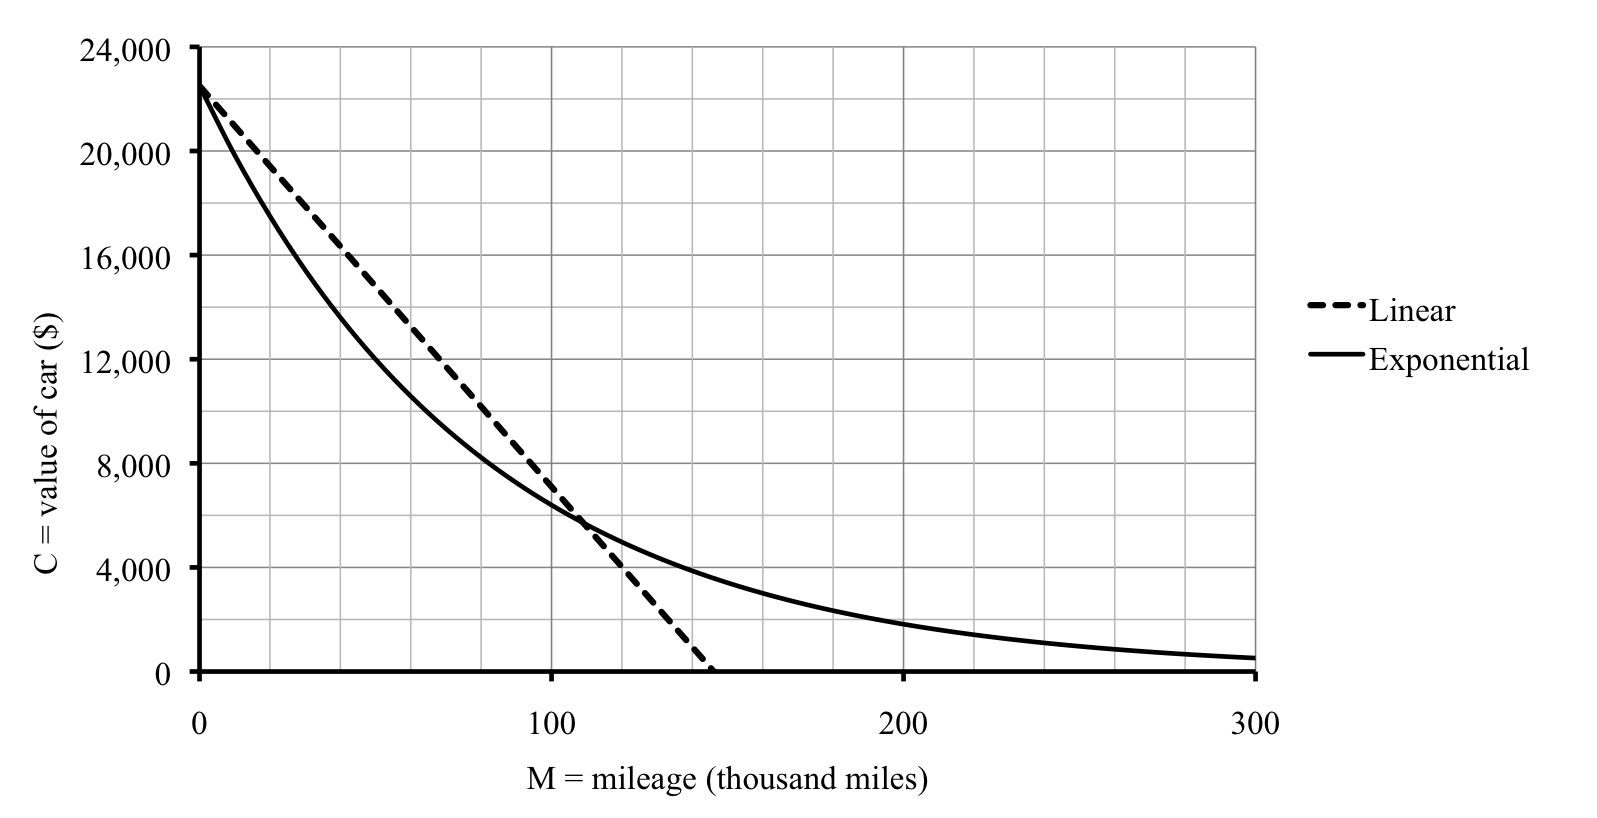
\includegraphics [width = 6in] {carvalue.png}}
\end{center}
There's no way of knowing whether the function is linear or exponential.  It is probably not exactly either one.  But if we have to pick, the exponential model seems closer to reality.  

 %\section{Linear vs.\ exponential models}

 \begin{center}
\line(1,0){300} %\line(1,0){250}
\end{center}

\section*{Homework}

\noindent \textbf{Start by doing Practice exercises \#1-4 in the workbook.}

\bigskip

\noindent \textbf{Do you know \ldots}

\begin{itemize}

\item When we might think a model might be linear? 
\item The template for a linear equation? 
\item How to find the linear equation between two points (a start and end value)? 

\item When we might think a model might be exponential? 
\item The template for an exponential equation? 
\item How to find the exponential equation between two points (a start and end value)? 

\item Why we compare linear and exponential models? 
 \item[~] \textbf{If you're not sure, work the rest of exercises and then return to these questions.  Or, ask your instructor or a classmate for help.} 
\end{itemize}

\subsection*{Exercises}

\begin{enumerate} 
\setcounter{enumi}{4}

\item 
\begin{enumerate} 
\item 
Gina weighed 165 pounds when she started her diet three months ago.  Now she weighs 153 pounds.  How much longer will she have to stay on her diet to reach her goal weight of 120 pounds?  Make an initial guess of how long it will take her, and use a linear and an exponential model to predict how long she will be on her diet.  \emph{That means, write both equations and solve each to find the answer.} 
\item Gina's diet-buddy Casey started at 253 pounds and now weighs 235 pounds after 3 months.  Casey's goal weight is 178 pounds.  How long will it take him?  Again, make an initial guess, and then use a linear and an exponential model to predict. \emph{Again, write and then solve both equations.}
\item Explain why weight loss might be similar to a car depreciating in value.  Think about what happens at the start of a diet and what happens long run.
\end{enumerate}

\item Chlorofluorocarbons (CFC) are greenhouse gases that result from our use of refrigeration, air conditioning, aerosols, and foams.  In 1960, the concentration of CFC in the northern hemisphere was 11.1 parts per trillion (ppt), meaning on average, there are 11.1 CFC molecules in a trillion molecules of air.  In 1980 the concentration was 177 ppt.  Use $C$ for the concentration in the northern hemisphere in ppt and $Y$ for the year, measured in years since 1960.  
\hfill \begin{footnotesize} U.S.\ Department of Energy \end{footnotesize}
%SOURCE?Info and links: %%% Enviromath in the classroom book, pg 22
%%% http://cdiac.ornl.gov/oceans/new_atmCFC.html
% That's from the Carbon Dioxide Information Analysis Center, part of DOE's Oak Ridge Labs.
\begin{enumerate}
\item Suppose that this concentration has been increasing at a \emph{constant rate each year}.
\begin{enumerate}
\item By how many parts per trillion per year have CFC concentrations increased?
\item Write an equation illustrating this model.
\item According to this equation, how much will the concentration of CFC be by the year 2015?
\item What type of equation is being used here?
\end{enumerate}
\item  Assume instead that the concentration of CFC has been increasing \emph{a fixed percentage each year}.
\begin{enumerate}
\item What is the annual growth factor that CFC concentrations increased?  
\item Write an equation illustrating this model.
\item According to this new equation, how much will the concentration of CFC be by the year 2015?
\item What type of equation is being used here?
\end{enumerate}
\end{enumerate}

\item According to an online calculator, the recommended daily caloric intake for a woman Diane's height, weight, and activity level was \text{1,900} calories/day when she was 30 years old and \text{1,840} calories per day when she was 40 years old.
\begin{enumerate}
\item Name the variables and summarize the information in a table.  Start her age at 30 years old (so you will know the intercept).
\item Use a linear model to estimate the recommended daily caloric intake for Diane when she was 20 years old and now that she's 50 years old.  According to this model, what will it be when she's 80 years old? \emph{Note:  because we started the age at 30 years old, you will need to use -10 to get her age of 20 years old.  Looks weird, but 20 is 10 years before our starting value 30 so officially that's a negative.  It works fine.}
\item Repeat using an exponential model instead.
\item Thoughts?
\end{enumerate}

\item In 1995 the average price of a movie ticket was \$4.35, and in 2011 the average price of a movie ticket was \$7.93.  The variables are $T$, the average price of a movie ticket in dollars and $Y$ the number of years since 1995.  

\hfill \begin{footnotesize} Source: National Association of Theatre Owners \end{footnotesize}
\begin{enumerate}
\item Write a linear equation that fits this information and use it to estimate the average price of a movie ticket in 2015 and 2025.
\item Write an exponential equation that fits this information and use it to estimate the average price of movie ticket in 2015 and 2025.
\item Draw a graph of each function on the same set of axes.  (Include also what each equation said about ticket prices in the year 2000.)
\item The actual average movie ticket price in the year 2000 was \$5.39.  Which model predicted a closer value -- linear or exponential?
\end{enumerate}

\item The number of asthma sufferers worldwide in 1990 was 84 million and 130 million in 2001.  Let $A$ be the number of people with asthma (in millions) and $Y$ the year, measured in years since 1990.  Compare what the linear and exponential models project for the year 2015 and 2030.  Include a graph showing both functions on the same axes.

\item  Sales of hybrid cars in the United States have continued to increase.  In 1999, 17 (yes, seventeen) hybrid cars were sold.  By 2002 that number was up to \text{34,521} hybrid cars sold. Write $H$ for the number of hybrid cars sold and $Y$ for the year, measured in years since 1999.  
\hfill \begin{footnotesize} Source: Earth Policy Institute \end{footnotesize}
%%% http://www.earth-policy.org/index.php?/data_center/C26/
\begin{enumerate}
\item Suppose that the hybrid car sales have been increasing \emph{at a constant rate each year.}  Write the appropriate equation and use it to estimate sales in 2011. 
\item Assume instead that hybrid car sales have been increasing \emph{a fixed percentage each year.} Write the appropriate equation and use it to estimate sales in 2011.  Comment.
\item Actual sales of hybrid cars in 2010 were around \text{13,500}.  Why might the number be lower than the linear model predicted?
\end{enumerate}  


\end{enumerate}